\documentclass{article}

\usepackage[english]{babel}
\usepackage{tgtermes}
\usepackage{xcolor}
\usepackage{pagecolor}
\usepackage{hyperref}
\usepackage{graphicx}
\usepackage[labelformat=empty]{caption} 
\usepackage{amsfonts}
\usepackage{booktabs}
\usepackage{siunitx}
\usepackage{adjustbox}
\usepackage{caption}
\usepackage{float}


% % DRACULA COLORS
% \definecolor{draculabg}      {RGB} {25,   25,   25}
% \definecolor{draculacl}      {RGB} {68,   71,   90}
% \definecolor{draculafg}      {RGB} {248,  248,  242}
% \definecolor{draculacomment} {RGB} {98,   114,  164}
% \definecolor{draculacyan}    {RGB} {139,  233,  253}
% \definecolor{draculagreen}   {RGB} {80,   250,  123}
% \definecolor{draculaorange}  {RGB} {255,  184,  108}
% \definecolor{draculapink}    {RGB} {255,  121,  198}
% \definecolor{draculapurple}  {RGB} {189,  147,  249}
% \definecolor{draculared}     {RGB} {216,  47,   49}
% \definecolor{draculayellow}  {RGB} {241,  250,  140}
% \definecolor{draculablue}  {RGB} {36,  85,  151}


% DEFAULTS
\definecolor{draculabg}      {RGB} {255, 255, 255}
\definecolor{draculacl}      {RGB} {0,0,0}
\definecolor{draculafg}      {RGB} {0,0,0}
\definecolor{draculacomment} {RGB} {0,0,0}
\definecolor{draculacyan}    {RGB} {0,0,0}
\definecolor{draculagreen}   {RGB} {0,0,0}
\definecolor{draculaorange}  {RGB} {0,0,0}
\definecolor{draculapink}    {RGB} {0,0,0}
\definecolor{draculapurple}  {RGB} {0,0,0}
\definecolor{draculared}     {RGB} {0,0,0}
\definecolor{draculayellow}  {RGB} {0,0,0}
\definecolor{draculablue}  {RGB} {0,0,0}

\pagecolor{draculabg}
\color{draculafg}

\nocite{*}

\title{\textbf{Aldone}}
\author{Fausto Zamparelli, Daniel Falbo}
\date{May 30, 2024}

\hypersetup{
colorlinks=true,
linkcolor=draculapurple,
citecolor=draculapurple,
urlcolor=draculapurple,
pdftitle={Aldone},
pdfpagemode=FullScreen,
}

\begin{document}

\maketitle

\section*{\color{draculagreen}Introduction}
Aldone as in "AI-Done" is a tool for personal reminders and grocery list management.
This is a proof of concept of a product that could save you time every day by allowing you
to smoothly interact with it on the fly.

Aldone is a react web app that interacts with a node.js and a python server doing most of the magic.
After a log-in you will be able to speak to it to add tasks to your grocery list, to-do list,
or make questions about reminders you saved earlier.
Furthermore, you could ask to split a task in sub-tasks or approximate how long a task will take.
Aldone is able to detect fully by himself weather you are asking him to add something to your grocery list or to-do list.

The coolest thing is that once you will come home from the supermarket with tired legs and arms from carrying bags, you won't have to manually remove everything from this digital grocery list but you can use your phone camera to detect what foods you actually bought and then Aldone will remove them for you. Other use cases for this include checking what's already in your kitchen or marking products as bought after delegating your groceries to someone else.

\newpage

\section*{\color{draculagreen}Method} 
\begin{figure}[htbp]
\centering
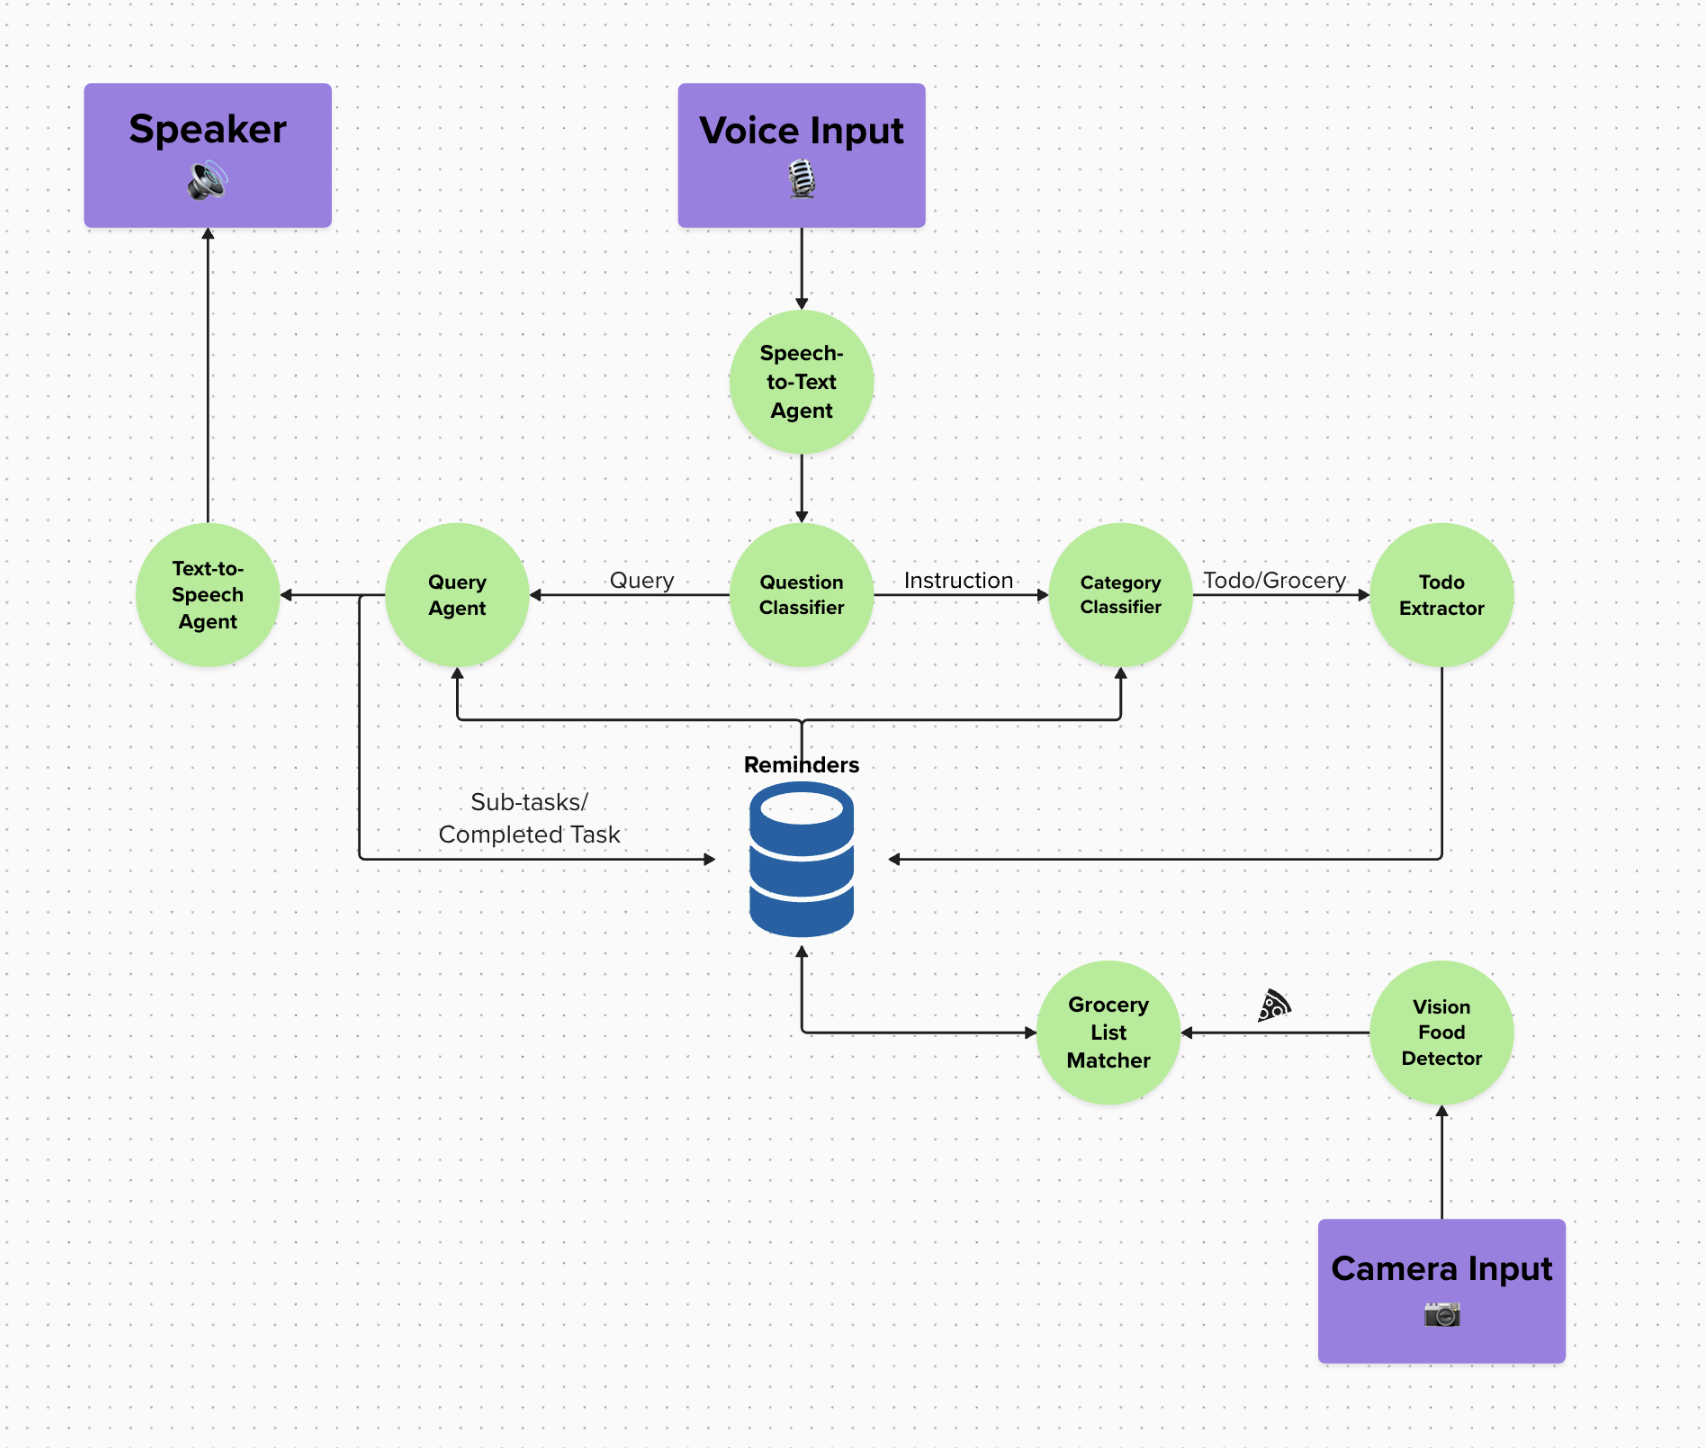
\includegraphics[width=\textwidth]{diagram.png}
\caption{\small Visual representation of the agents that make up Aldone}
\end{figure}

As we can see Aldone was created by splitting its behind-the-scenes functionalities into multiple specialized AI agents that cooperate with each others. In order to fully understand how Aldone works under the hood it is best to understand the functionality of each of these agents alone. Let's work our way thorough the graph from top to bottom:

\subsection*{\color{draculayellow}Speech-to-Text Agent}
For the Speech-to-Text task, being a web app, Aldone uses the browser's built-in Web Speech API service for convenience. The implementation can be found by searching for ``webkitSpeechRecognition" in the `src/app/[username]/page.tsx' file.

\newpage

\subsection*{\color{draculayellow}Question Classifier}
The task of the Question Classifier is to determine whether the user's input is a question/query or a statement/instruction. Anything that involves looking for information in the web or from the existing data in the database, is a query. Anything that provides new data within the input, is not a query.

\begin{figure}[H]
\begin{center}
\begin{tabular}{SS}
  \toprule
    \text{Input} & \text{Label} \\
    \midrule
    \text{``What's the capital of Italy?"}  & \text{Query} \\
    \text{``Add milk to my grocery list"}  & \text{Not Query}  \\
    \text{``Split task X into subtasks"} & \text{Query}  \\
    \bottomrule
\end{tabular}
\end{center}
\caption{\it For example, the input "What's the capital of Italy?" is a query, while "Add milk to my grocery list" is an instruction. The input "Split task X into subtasks" is also a query because the data is not being provided by the input.} \label{faketable:mul}
\end{figure}


The Question Classifier is implemented using a neural network trained on a dataset of 500 examples. The dataset was manually generated and enhanced using generative AI data synthesizing tools. The question classifier is a pytorch neural network and its code can be found in the subdirectory ``src/py/question\_classifier''.

In the subdirectory,
\begin{itemize}
 \item \texttt{nndata.json}: is the dataset used to train the model
  \item \texttt{nntraining.py}: is the training script that generates the model. 80\% of the data is used for training and 20\% for testing. Of the training data, 25\% is used for validation.
  \item \texttt{nnlabeler.py}: uses the trained model to label new input data.
\end{itemize}

\begin{figure}[htbp]
\centering
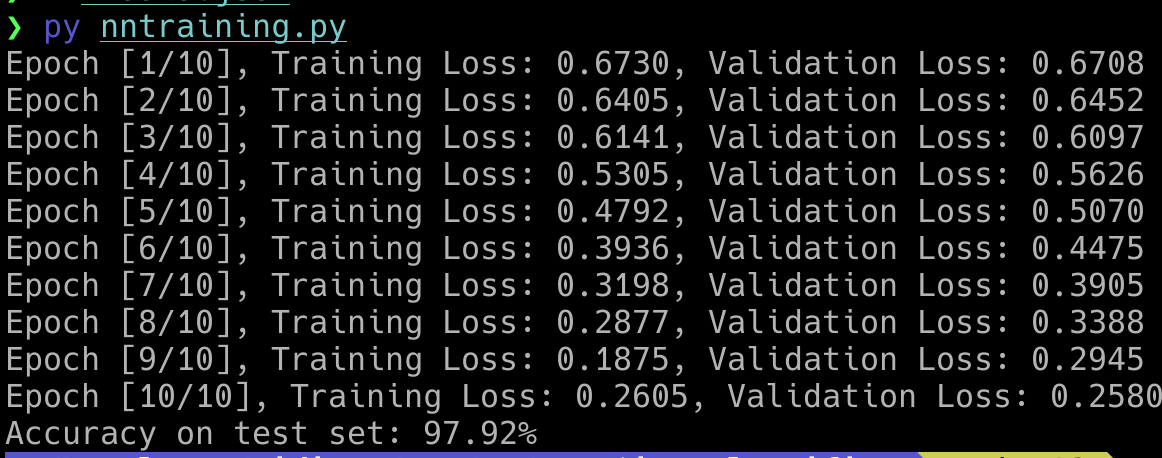
\includegraphics[width=\textwidth]{question_classifier_accuracy.png}
\caption{\small The model achieved 98\% accuracy on the test set. Of course it's still a small dataset and more data would make it more solid.}
\end{figure}

\subsection*{\color{draculayellow}Category Classifier}

The task of the category classifier is to classify wheter the input to-do belongs to the reminders list or the grocery list. To achieve this, an intent classification dataset from Hugging Face was used. The data looked like this:

\begin{figure}[H]
\begin{center}
\begin{tabular}{SS}
  \toprule
    \text{Input} & \text{Label} \\
    \midrule
    \text{``tell me how to set up a direct deposit"}  & \text{direct\_deposit} \\
    \text{``switch to whisper mode"}  & \text{whisper\_mode}  \\
    \text{``i'm out of lysol could you order me some"}  & \text{order}  \\
    \text{``set my alarm for 5pm"}  & \text{alarm}  \\
    \text{``can you list my shopping list for me"}  & \text{shopping\_list}  \\
    \text{``update my shopping list, delete canned olives"}  & \text{shopping\_list\_update}  \\
    \text{``can you list my shopping list for me"}  & \text{shopping\_list}  \\
    \text{``remove laundry from my todo list"}  & \text{todo\_list\_update}  \\
    \text{``i want to hear everything on my todo list"}  & \text{todo\_list}  \\
    \bottomrule
\end{tabular}
\end{center}
\end{figure}

The cagory classifier is trained on the whole dataset but only the labels that are relevant are used: shopping\_list and shopping\_list\_update direct the flow to the grocery list, while todo\_list and todo\_list\_update direct the flow to the to-do list. The category classifier is a scikit-learn Naive Bayes classifier and its code can be found in the subdirectory ``src/py/todo\_classifier''.


In the subdirectory,
\begin{itemize}
  \item \texttt{train\_classifier.py}: is the training script that fetches the data from hugging face and then trains and exports the model as a raw python object with pickle. The dataseta was already partitioned by train/test/validation sets by hugging face.
  \item \texttt{use\_classifier.py}: uses the saved model python object to label new input data.
\end{itemize}

\subsection*{\color{draculayellow}Todo Extractor}

The task of the Todo Extractor is to extract the task from the user's input. For example, if the user says "Add milk to my grocery list", the task is "Add milk". The Todo Extractor is implemented using OpenAI's pre-trained GPT 3.5 model.

The prompt used was
\begin{verbatim}
`The following is a voice command recorded form
a voice assistant, extract the todo item from it to
insert it in a todo list.  For example, if the voice command
is 'Add 'Buy milk' to my shopping list', the extracted todo item
is 'Buy milk'.  You should also generate a "nice_readable_id"
and finally return a json object structured
exacly as {text: string; id: string}.
For example, {text: 'Buy milk', id: 'milk_buy'}.`
\end{verbatim}

This allowed to have nice json objects as output that are much easier to work with programmatically.

The code can be found in the subdirectory ``src/app/api/todoExtractor''.


\subsection*{\color{draculayellow}Vision Food Detector}

The task of the Vision Food Detector is to take a video stream and detect food items in it. The Vision Food Detector is implemented using a pre-trained YOLO model via Ultralytics and filtering the detected items to a set of labels containing only foods. The code can be found in the subdirectory ``src/py/grocery\_recognition''.

IMAGE HERE

\subsection*{\color{draculayellow}Grocery List Matcher}

The task of the Grocery List Matcher is to take the items detected by the Vision Food Detector and cross them out from the grocery list. Like the Todo Extractor, the Grocery List Matcher is implemented using OpenAI's pre-trained GPT 3.5 model.

The prompt used was
\begin{verbatim}
`The following are the products that were
seen on the table: <products array>

The following is a json array of grocery list items
structured like [{text: string, completed: bool, id: string}].
Return me a json array of grocery list items ids of items that
were also seen on the table, if any.

Even if the ids don't match exactly, you can still match
them if they are similar. For example, if the table has "apple"
and the grocery list has "red_apple", you can still match them.
Be smart and human about it. Make sure to return the id
as seen in the "id" field of the grocery list item,
not the products seen on the table.

The result should be formatted
like {ids: ["red_apples", "berries"]}.
If none of the items were seen on the table,
return an empty array "{ids: []}".       

<grocery list object>
`
\end{verbatim}

The code can be found in the subdirectory ``src/app/api/groceryListMatcher''.

Initially the LLM model was asked to output the entire updated grocery list object, but empirically it made errors very often. Asking the LLM model for ids of the grocery list that were updated, and then updating the grocery list object programmatically, ended up working much better.

\subsection*{\color{draculayellow}General Agent}

\subsection*{\color{draculayellow}Text-to-Speech Agent}

\section*{\color{draculagreen}Results}

\subsection*{\color{draculagreen}Glue Orchestration}

\section*{\color{draculagreen}Source of inspiration}

[1] \href{https://humane.com/media/cosmos-an-operating-system-for-the-ai-era}{Cosmos: An Operating System for the AI Era} \newline
[2] aiXplain

\end{document}
